\paragraph[]{Entity Relationship Diagram} \hspace{1cm} \par
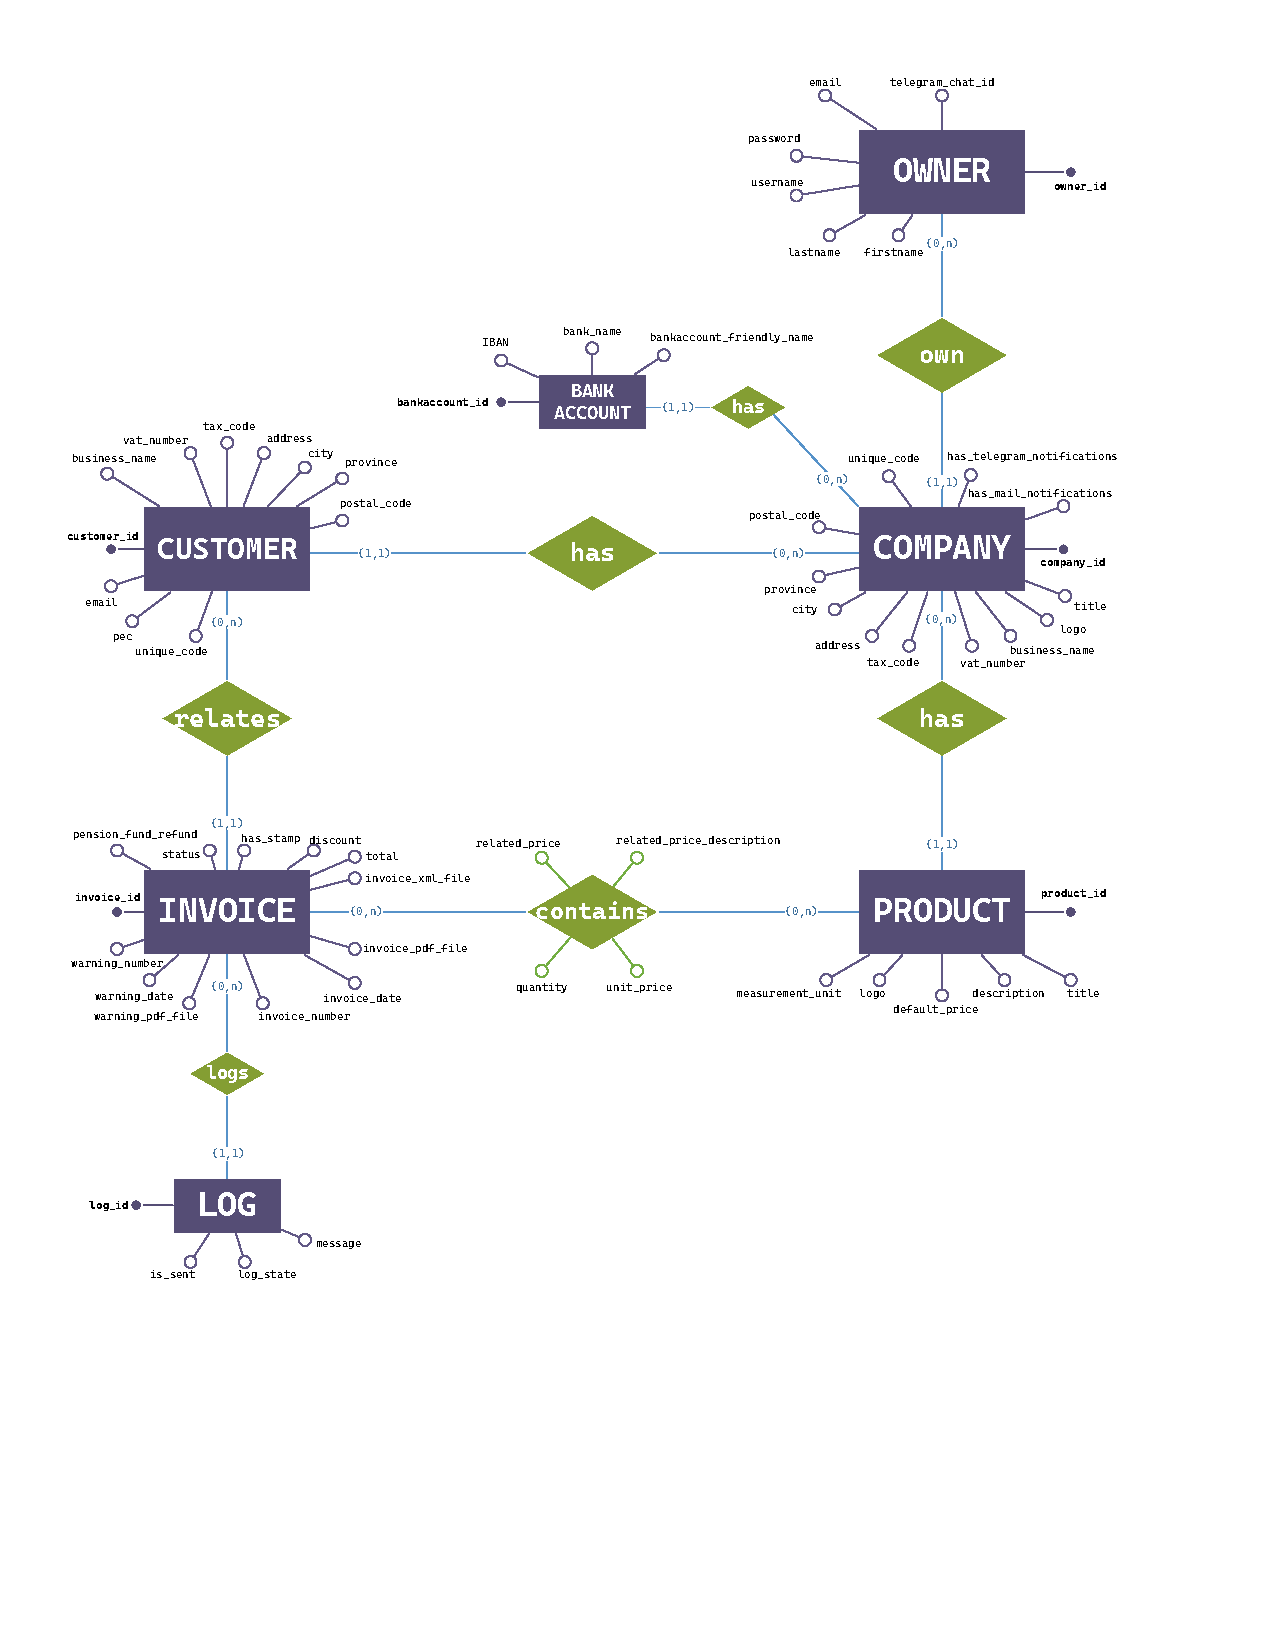
\includegraphics[width=\textwidth, keepaspectratio]{resources/ERSchema.pdf}
\vspace{8mm}
%Describe here your ER schema


The Entity-Relationship schema is composed of the following entitites:
\begin{itemize}
 	\item Owner: contains the informations about the owner of one or more companies that are registered in the system. The primary key owner\_id is an auto-increment (serial) integer ID. The other attributes are firstname (char), lastname (char), username (char), password (char), email (char) and telegram\_chat\_id (char).
	\item Company: contains the informations about a company that is registered in the system. The primary key company\_id is an auto-increment (serial) integer ID. The other attributes are title (char), logo (char), business\_name (char), vat\_number (char), tax\_code (char), address (char), city (char), province (char), postal\_code (char), unique\_code (char), has\_telegram\_notifications (boolean), has\_mail\_notifications (boolean). Then, owner\_id (integer) is an external key pointing to the primary key of the entity Owner, indicating the owner of the company.
	\item BankAccount: contains the information about the bank account of a company. The primary key bankaccount\_id is an auto-increment (serial) integer ID. The other attributes are IBAN (char), bank\_name (char), bankaccount\_friendly\_name (char). Then, company\_id (integer) is an external key pointing to the primary key of the entity Company, indicating the company owning to the bank account.
   	\item Customer: contains the informations about a customer/client of a company. The primary key customer\_id is an auto-increment (serial) integer ID. The other attributes are business\_name (char), vat\_number (char), tax\_code (char), address (char), city (char), province (char), postal\_code (char), email (char), pec (char), unique\_code (char). Then, company\_id (integer) is an external key pointing to the primary key of the entity Company, indicating the company that has the customer as a client.
   	\item Product: contains the informations about a product or a service sold by a company. The primary key product\_id is an auto-increment (serial) integer ID. The other attributes are title (char), default\_price (integer), logo (char), measurement\_unit (char), description (char). Then, company\_id (integer) is an external key pointing to the primary key of the entity Company, indicating the company that sells the product.
	\item Invoice: contains the informations about an invoice that is being generated and modified or has been already emitted. The primary key invoice\_id is an auto-increment (serial) integer ID. The other attributes are status (integer), warning\_number (char), warning\_date (date), warning\_pdf\_file (char), invoice\_number (char), invoice\_date (date), invoice\_pdf\_file (char), invoice\_xml\_file (char), total (double), discount (double) pension\_fund\_refund (double), has\_stamp (boolean). Then, customer\_id (integer) is an external key pointing to the primary key of the entity Customer, indicating the customer to which the invoice will be billed and sent.
	\item Log: contains the logs of an invoice and of the process of creating and modifying the invoice. The primary key log\_id is an auto-increment (serial) integer ID. The other attributes are is\_send (boolean), log\_state (boolean), message (char). Then, invoice\_id (integer) is an external key pointing to the primary key of the entity Invoice, indicating the invoice to which the log is related.
\end{itemize}
Every one of this entities corresponds to a table in the sql schema.

The relation InvoiceProduct defines the products listed in an invoice and has the following attributes: quantity (integer), unit\_price (double), related\_price (double), related\_price\_description (char) and purchase\_date (date). The relation, in the sql schema, is translated into a table that has as primary key the union of invoice\_id, an external key which points to the invoice which the invoiceProduct is part of, and product\_id, an external key which points to the product which the invoiceProduct relates to.


